\section{Lezione 1}

\begin{defn}[Carica elettrica]
	La carica elettrica \emph{Q} è una proprietà fondamentale della materia che indica il passaggio di corrente elettrica per tempo: $$ \SI{1}{C} = \SI{1}{\ampere\second} $$ \\
	La carica elettrica può essere sia positiva sia negativa, ed è quantizzata, cioè tutte le cariche sono multipli della carica elementare: $$ q = \SI{1.6021e-19}{C} $$  
	Le cariche elettriche sono sempre soggette ad una forza elettrica, detta \emph{di Coulomb}, pari a $$ \vec{F} = \frac{1}{4\pi\varepsilon} \cdot \frac{q_1 q_2}{r^2} \cdot \hat{r} $$
\end{defn}

\begin{defn}[Corrente elettrica]
	La corrente elettrica, o intensità di corrente elettrica, \emph{I}, è data dal movimento di cariche mobili e matematicamente si esprime come la derivata della carica elettrica rispetto al tempo: $$ I = \frac{dQ}{dt} $$
	La corrente si misura in serie con l'amperometro.
\end{defn}

\begin{defn}[Differenza di potenziale]
	La tensione \emph{V} tra due punti è l'integrale di linea del campo elettrico su un percorso qualsiasi che congiunga i due punti: $$ V_{ab} = \int_a^b \vec{E} \cdot \vec{dl} $$
	La tensione si misura in parallelo con il voltmetro.
\end{defn}

\begin{defn}[Potenza]
	La potenza \emph{P} è il prodotto tra la tensione e la corrente: $$ P = V I $$
	La potenza si misura in watt. Ha segno positivo se il bipolo aumenta l'energia immagazzinata, negativo se la diminuisce.
\end{defn}

\begin{defn}[Energia elettrica]
	L'energia elettrica viene distribuita attraverso la rete di distribuzione con un sistema trifase a quattro conduttori: tre hanno tensioni sinusoidali sfasate tra loro di $\frac{2\pi}{3}$, il quarto, detto neutro, è collegato a terra e costituisce il potenziale zero di riferimento. Il valore medio della tensione di rete è zero, mentre il valore efficace (root-mean-square rms) è 230 V. 
	Le apparecchiature elettriche devono rispettare determinate specifiche di sicurezza: 
	\begin{itemize}
		\item classe I: messa a terra di protezione \\
		un circuito elettrico monofase ha tutte le parti in tensione isolate per il livello di tensione nominale, mentre l'involucro metallico dell'apparecchiatura è collegato a terra. Inoltre, sono posizionati due interruttori differenziali (o salvavita) che rilevino lo squilibrio tra la corrente di fase e la corrente di guasto. Un interruttore differenziale deve aprire il circuito quando la differenza tra le correnti è maggiore o uguale a 30 mA, cioè la soglia di pericolosità della corrente per il corpo umano. 
		\item classe II: doppio isolamento \\
		Gli apparecchi a doppio isolamento non richiedono la messa a terra e sono costruiti in modo che un singolo guasto non possa causare il contatto con tensioni pericolose.
		\item classe III: bassissima tensione di sicurezza \\
		Una tensione non superiore a 25 V in alternata o 50 V in continua non rappresenta un pericolo per il corpo umano. Si consiglia di non superare il $\pm$ 12 per i circuiti che vedremo in laboratorio. 
	\end{itemize}
\end{defn}

\begin{defn}[Bipoli elettrici]
	I circuiti elettrici sono formati da elementi circuitali interconnessi tra di loro. I più semplici elementi circuitali sono dispositivi a due terminali, o bipoli. \\
	Al bipolo è applicata la differenza di potenziale \emph{V} e attraverso di esso fluisce la corrente elettrica \emph{I}. I due terminali vengono contrassegnati con i simboli \emph{+} ed \emph{-}. 
	La tensione si misura dal polo negativo a quello positivo. La corrente si considera positiva quando entra nel bipolo \emph{+}. 
\end{defn}

\begin{defn}[Nodo]
	Un nodo è un punto di un circuito elettrico in cui si incontrano due o più bipoli.
\end{defn}

\begin{defn}[Maglia]
	Una maglia è un percorso chiuso attraverso due o più bipoli di un circuito.
\end{defn}

\begin{defn}[Resistore e legge di Ohm]
	Il più semplice bipolo lineare è il resistore, caratterizzato da proporzionalità diretta tra tensione e corrente (\emph{Legge di Ohm}): 
	$$ V = R I $$ dove R è la resistenza che si misura in Ohm: $$ 1 \Omega = 1 V/A = 1 kg m^2 / (A^2 s^3) $$
\end{defn}

\begin{defn}[Generatori]
	Un generatore è un bipolo attraverso 
	Un generatore di tensione presenta una tensione fissata fra i suoi terminali. Il più semplice generatore di tensione constante nel tempo è una pila o batteria. 
\end{defn}

\begin{defn}[Multimetro]
	Un multimetro è uno strumento di misurazione in grado di misurare tensione, corrente e resistenza. I multimetri possono essere analogici e digitali, palmari o da banco. \\
	La corrente (sia in alternata sia in continua) si misura in serie, quindi bisogna aprire il circuito ed inserire l'amperometro in serie. \\
	La tensione (sia in alternata sia in continua) si misura in parallelo, quindi bisogna mettere in parallelo il voltmetro. Misurare la tensione è più comodo rispetto alla misura di corrente. \\
\end{defn}

\begin{defn}[Alimentatore]
	Un alimentatore funziona in modo simile ad un generatore ideale e forniscono una differenza di potenziale di circa 30 V. Se vogliamo una corrente o positiva o negativa, si effettua manualmente un collegamento a terra tra il terminale e l'alimentatore. 
\end{defn}

\begin{defn}[Partitore di tensione]
	Un partitore di tensione è costituito da due o più componenti passivi collegati in serie. Se ai capi della serie viene applicata una tensione, essa si ripartirà ai capi dei componenti in base al loro valore. 
\end{defn}


\begin{defn}[Cortocircuito]
	Il cortocircuito è un collegamento tra due nodi effettuato con un generatore di tensione nulla. In un cortocircuito la tensione ai capi del generatore è nulla, quindi la corrente può assumere qualsiasi valore.
\end{defn}

\begin{defn}[Circuito aperto]
	Un generatore di corrente spento è percorso da una corrente nulla e tensione qualsiasi.
	Il circuito aperto è un collegamento tra due nodi effettuato con un generatore di corrente nulla.
\end{defn}

\begin{defn}[Leggi di Kirchhoff]
	La somma algebrica delle correnti in un nodo di un circuito è zero: $$ \sum_{i} I_i = 0 $$
	La somma algebrica delle tensioni in una maglia di un circuito è zero: $$ \sum_{j} V_j = 0 $$
\end{defn}

\begin{defn}[Partitore di tensione]
	Un partitore di tensione è costituito da due o più componenti passivi collegati in serie.
	Se ai capi della serie viene applicata una tensione, essa si ripartirà ai capi dei componenti in base al loro valore.
	\begin{figure}[H]
		\centering
		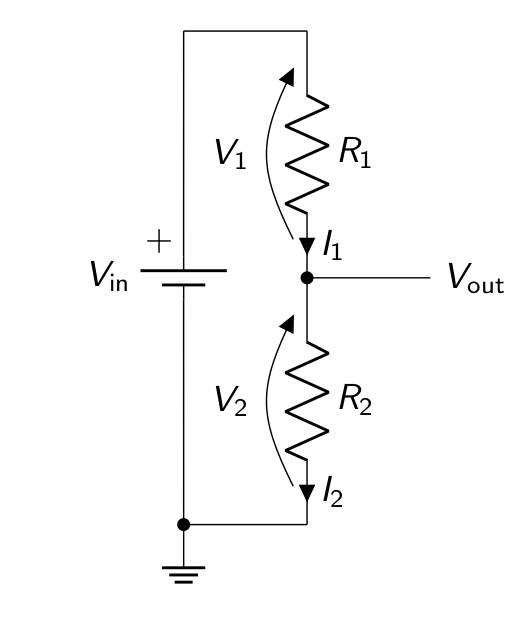
\includegraphics[width=0.5\linewidth]{figures/partitore_tensione.png}
		\caption{Partitore di tensione}
		\label{fig:partitore_tensione}
	\end{figure}
\end{defn}

